%%%%%%%%%%%%%%%%%%%%%%%%%%%%%%%%%%%%%%%%%%%%%%%%%%%%%%%%%%%%%%%

\chapter{Results}
\label{chap:results}

\section{Introduction}

Since the sensitivity of the analysis is much lower than the SM prediction, the reported results set upper limits on the branching fraction for the \Hee decay. To do so, a likelihood fit of the signal and background models to the \mee distributions is performed in all analysis categories simultaneously. The fitted parameters are then used to extract observed and expected limits at various confidence levels. 

In the following chapter, the construction of the likelihood is presented, alongside the corresponding signal-plus-background fits to \mee distributions. The results of the analysis comprise limits on \BHee for a selection of Higgs boson masses, as well as per analysis category.


\section{The likelihood function}
In order to extract upper limits on the \Hee branching fraction, this analysis uses a binned simultaneous maximum likelihood fit to the \mee distributions in data over all analysis categories.
The fit is performed over the the range $110<\mee<150$~GeV, with bin widths of 0.25~GeV, chosen to be as small as possible to prevent information loss. In this case, the likelihood is proportional to the product of Poisson terms over count observations from all bins in the \mee distribution. For a given category, the likelihood, $\mathcal{L}_{c}$, is expressed as: %note than mu is not the BR. Its the scaler of the BR.

\begin{equation}
    \mathcal{L}_{c}(\mathrm{data}|\vec{\mu},\mH,\vec{\theta}) = \prod_{i}^{N_{b}} \mathrm{Poisson} \left( d_{i} \, \Big| \left[ s_{i}(\vec{\mu},\mH,\vec{\theta_{s}}) + b_{i}(\vec{\theta_{b}}) \right] \right),
\end{equation}
%In this formalism, the analysis can be expressed as a combination of many counting experiments. Each experiment...etc.
%For each bin, $i$, there is a probability of seeing the observed value in Data, given the expected (from the S+B model), governed by a Poisson distribution. The likelihood of all observations is then proportional simply to the product of Poisson terms over all bins]. 

\noindent where $\vec{\mu}$ are the parameters of interest. The quantities $\vec{\theta_{s}}$ and $\vec{\theta_{b}}$ are the set of nuisance parameters affecting signal and background models respectively, which may be discrete or continuous ($\vec{\theta}=\{\vec{\theta_{s}},\vec{\theta_{b}}\}$). For the $i^{th}$ bin in the \mee distribution, of which there are $N_{b}$ total bins, the associated Poission term is composed of:

\begin{itemize}
    \item the \textit{observed} number of events in data, denoted by $d_{i}$, in bin $i$,
    \item the \textit{expected} number of events, obtained from the sum of signal and background yields, $s_{i}$ and $b_{i}$ respectively. The expected number of signal events depends on the POIs being tested, the Higgs boson mass, and the set of nuisance parameters affecting signal models. The background expectation is simply a function of the (unconstrained) nuisance parameters affecting the functional form and overall choice of background model. %so you have discrete ones i.e. choice of function and shape ones e.g. slope of one of the exponential fits or sth. Note also that a log-normal tends to a normal when the size of uncertainty/systemic (the sigma in the log normal) is small.
\end{itemize}



\noindent Since each analysis category contains an exclusive set of events, the final likelihood describing all events is obtained by taking the product over all per-category likelihoods

\begin{equation}
    \mathcal{L}(\mathrm{data}|\vec{\mu},\mH,\vec{\theta}) = \prod_{c}^{N_{c}} \left[\mathcal{L}_{c}(\mathrm{data}|\vec{\mu},\mH,\vec{\theta})\right] \cdot \Lambda({\vec{\theta}}),
\end{equation}

\noindent where $N_{c}$ is the number of analysis categories, and $\Lambda({\vec{\theta}})$ is the constraint term. For background models, the constraint adds a penalty in the likelihood for background candidates with large numbers of free parameters, to prevent fitting overly complex models. For nuisances affecting signal models, the term penalises deviations from the nominal nuisance parameter values. To prevent the signal yield becoming negative, the constraint terms on $\vec{\theta_{s}}$ that affect the normalisation are modelled using a log-normal distribution. %some are also gaussian. Background parameters have no constraint/prior since no a-priori knowledge about their range/interval is known

During the fit, the value of twice the negative logarithm of the likelihood is minimised using a numerical minimisation tool~\cite{RooFit}. The transformations to the likelihood are monotonic and do not change the resulting minima; they are performed to make the numerical minimisation task easier. The set of parameters which minimise the value of the 2NLL, for a given $\vec{\mu}$ being tested, are referred to as \textit{best-fit}. 
Since the \Hee analysis aims to set a limit on a single POI which scales the \BHee for each value of \mH, the replacement $\vec{\mu}\rightarrow\mu$ will be made in the notation from here on.



\section{Hypothesis testing and exclusion limits}
Setting limits on parameters of interest can be interpreted in the context of hypothesis testing. In the case of the \Hee search, the set of all possible values of the POI that scale the signal yield form a set of null hypotheses. The objective is to use the observed data to reject these hypothesis at various confidence levels. The CL is specified by the \textit{size} of the test, $\alpha$, which corresponds to the probability to reject the null hypothesis, even if it was true. 
%The interpretation of an exclusion limit set at the $100(1-\alpha)\%$ confidence level follows the frequentest paradigm, in that for a series of identical pseudoexperiments, the statement made about POI(s) should be correct $100(1-\alpha$)\% of the time. The choice for $\alpha$ depends on the hypothesis to be excluded, but is commonly chosen as 0.05.  %choice depends on how well separated the null and alternate hypothesis are. Lower alpha means more separation.

In order to set upper limits, a test statistic which summarises the observed data in a single value, $t_{\mu}$, is used. Typical test statistics often use ratios of likelihood functions constructed under a null and alternative hypothesis for $\mu$, since these maximise the \textit{power} of the test for a given test size, and have useful asymptotic properties~\cite{Cowan,NeymanPearson}. The test statistic distribution, $f(t_{\mu},\vec{\theta})$, is constructed for each considered value of $\mu$. The observed value of $t_{\mu}$ in data, $t_{\mu}^{obs}$, can then be used to compute a $p$-value; comparing the $p$-value with the chosen confidence level informs whether the null hypothesis under test can be excluded. For this analysis, the chosen test statistic is given by:

\begin{equation}\label{eqn:hee_test_stat}
     t_{\mu} =
    \begin{cases}
      -2\log\mathcal{L}(\mu,\mH,\hat{\vec{\theta}}_{\mu}) + 2\log\mathcal{L}(0,\mH,\hat{\vec{\theta}}_{0}), & \hat{\mu}<0;\\
      -2\log\mathcal{L}(\mu,\mH,\hat{\vec{\theta}}_{\mu}) + 2\log\mathcal{L}(\hat{\mu},\mH,\hat{\vec{\theta}}), & \hat{\mu}<(0,\mu];\\
      0, & \hat{\mu}>\mu,\\
    \end{cases} 
\end{equation}


\noindent where $\hat{\mu}$ and $\hat{\vec{\theta}}$ are the global best fit value of $\mu$ and ${\vec{\theta}}$ respectively, for all values of $\mu$ tested, while $\hat{\vec{\theta}}_{\mu}$ are the best-fit values of $\vec{\theta}$ for the current tested POI value, $\mu$. The test statistic has three regimes. The first case prevents unphysical values of $\hat{\mu}<0$, while the third imposes an upper limit on $\mu$. The second is equivalent to the ratio of log-likelihoods, constructed under the tested value of $\mu$, the null hypothesis, and under the best fit value, $\hat{\mu}$, the alternative hypothesis. The distribution of the test statistic can be determined analytically or from pseudo experiments. %to be concrete, the hypothesis is manifested in the (S+)B models

In this analysis, the $\mathrm{CL}_s$ procedure~\cite{CLs1,CLs2,LHCStatProcedures} is used to set exclusion limits. This method uses the distribution of the test statistic to compute a ratio of $p$-values, obtained from integrating $t_{\mu}$ under two hypotheses: the signal-plus-background ($\mu\neq0$), and background-only ($\mu=0$) scenarios. It is expressed as: %but these two hypothesis are not being compared to each other, they are being compared to the best fitting mu!

\begin{align*}
    CL_{s} &= \frac{p_{s+b}}{1-p_{b}}\\
           &= \frac{\int_{t_{\mu}^{obs}}^{\infty} f(t_{\mu}|\mu,\vec{\theta}=\hat{\vec{\theta}}_{\mu}^{obs})dt_{\mu}}{\int_{t_{0}^{obs}}^{\infty} f(t_{\mu}|0,\vec{\theta}=\hat{\vec{\theta}}_{0}^{obs})dt_{\mu}},
\end{align*}

\noindent where the nuisance parameters are set to their best-fit values for the chosen $\mu$ being tested. The $CL_{s}$ ratio is designed to make the test more conservative, avoiding excluding values of $\mu$ where the data also does not favour the background-only hypothesis. The smallest value of $\mu$ which satisfies $CL_{s}<\alpha$ is quoted as the upper limit on $\mu$, at the $1-\alpha$ confidence level. 

\section{Limits on \BHee}

This analysis reports exclusion limits on the branching fraction for \Hee decays at the 95\% confidence level ($\alpha$ = 0.05), for a selection of Higgs boson mass hypotheses between 120 and 130~GeV. Example \mee distributions, along with corresponding signal-plus-background models, are shown for the highest $S/B$ categories targeting \ggH and VBF events in Figure~\ref{fig:hee_S_plus_B_plots}, for a \Hee branching fraction scaled to the observed limit (at the 95\% CL), and assuming a Higgs boson mass of 125.38~GeV~\cite{CMS_Hgg_Hmass}. 

\begin{figure}[htbp!]
\centering
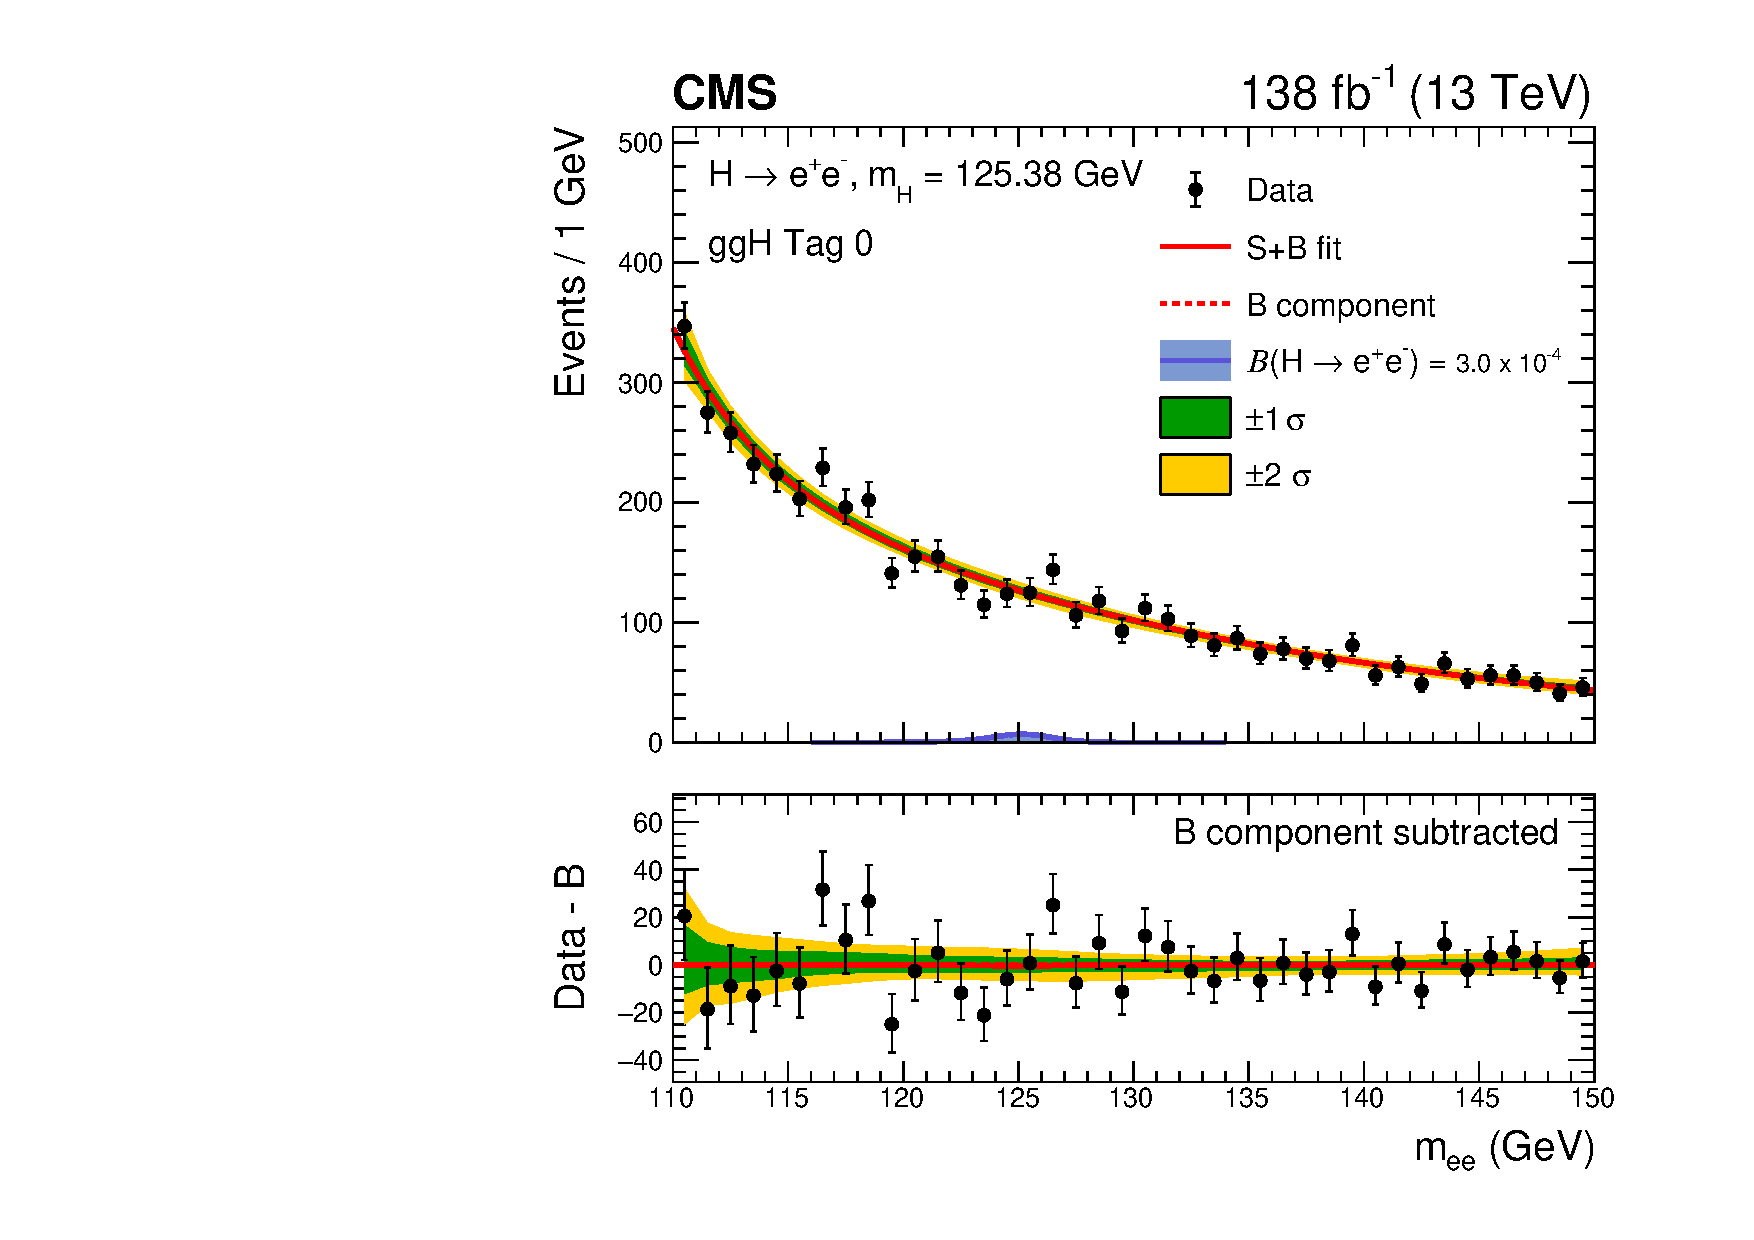
\includegraphics[width=0.49\textwidth]{Figures/Hee/Results/SPlusBModels/gghcat0_CMS_hgg_mass_paper.pdf}\hfill%
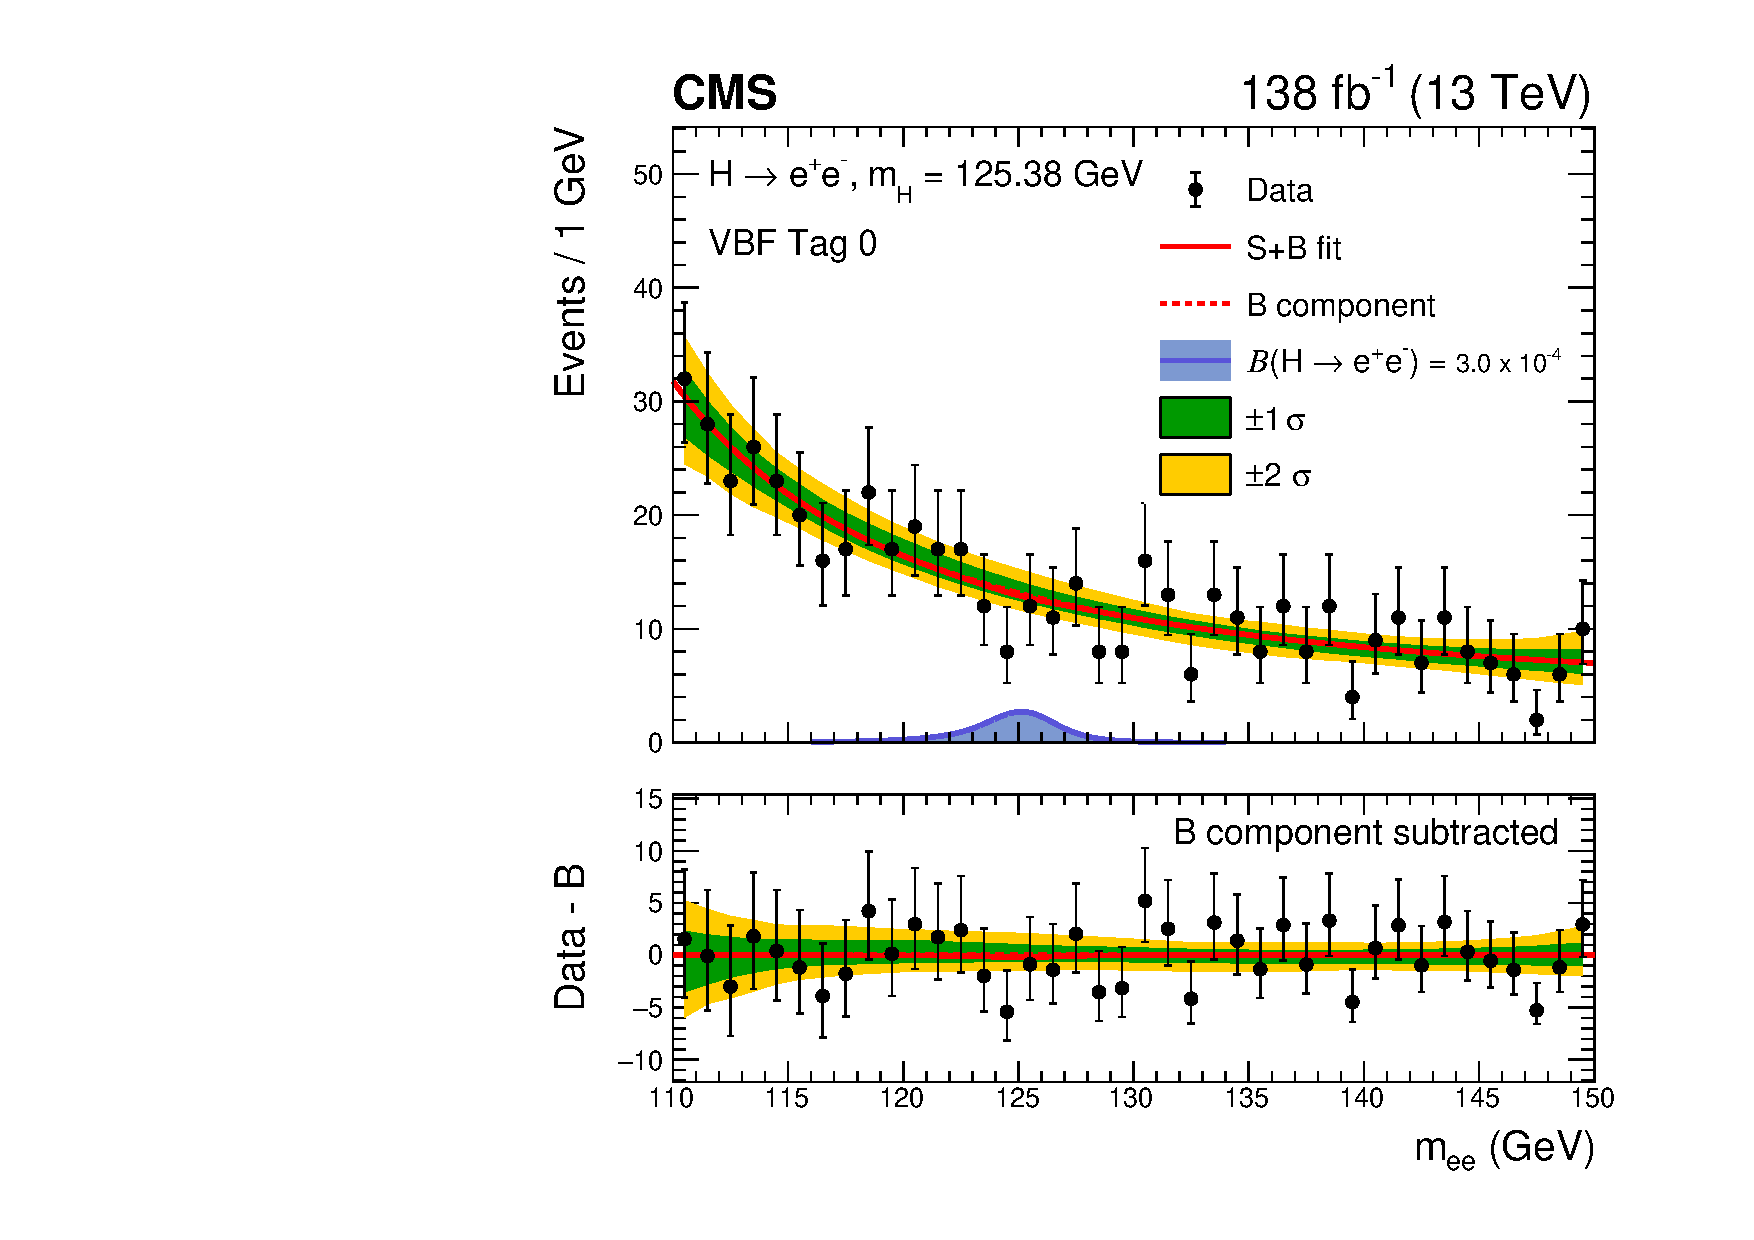
\includegraphics[width=0.49\textwidth]{Figures/Hee/Results/SPlusBModels/vbfcat0_CMS_hgg_mass_paper.pdf}\hfill%
\caption[The observed dielectron invariant mass distribution for the \ggH Tag 0 and VBF Tag 0 analysis categories.]{The signal-plus-background model fit (solid red line) to the \mee distribution for the highest $S/B$ analysis categories targeting the \ggH (left) and VBF (right) processes. The background-only component is also shown (dashed red line). The signal model for each category is shown (blue), scaled to the observed limit at $\mH=125.38$~GeV. The one (green) and two (yellow) standard deviation bands show the uncertainties in the background component of the fit. The lower panel shows the residual difference after subtraction of this background component.}
\label{fig:hee_S_plus_B_plots}
\end{figure}

Exclusion limits on \BHee are presented in Figure~\ref{fig:hee_limits}, for selected values of the Higgs boson mass. At the current best measured value of $\mH=125.38$~GeV~\cite{CMS_Hgg_Hmass}, the observed 95\% CL limit is

\begin{equation}
   \BHee < 3.0\times 10^{-4},
\end{equation}

\noindent while the expected limit is (also) $\BHee < 3.0\times 10^{-4}$. The p-value for this fit is 90\%, indicating good compatibility with the SM prediction. Limits at alternative Higgs boson mass points are of similar magnitude, with the observed limit consistently within the $1\sigma$ uncertainty interval of the expected value.  Limits are presented for each analysis category independently in Figure~\ref{fig:hee_limits_per_cat}, where it can be seen that the overall expected sensitivity is driven equally by \ggH and VBF categories.

Finally, the limit on the \Hee branching fraction is translated into an upper bound on the effective coupling modifier to electrons, $|\kappa_{e}|$. The coupling modifier is defined as the ratio of the observed electron-Yukawa coupling, to the SM prediction, $|\kappa_{e}|=|Y_{e}^{obs}|/|Y_{e}^{\mathrm{SM}}|$, such that deviations from $|\kappa_{e}|=1$ indicate non-SM behaviour. It is related to the \Hee branching fraction by

\begin{equation}
    \BHee = \frac{|\kappa_{e}|^{2} \BHee_{\mathrm{SM}}}{1+(|\kappa_{e}|^{2}-1)\BHee_{\mathrm{SM}}},
\end{equation}

\noindent where $\BHee_{\mathrm{SM}}$ is the \Hee branching fraction predicted by the SM. At a nominal Higgs boson mass of $\mH=125.38$~GeV, an upper limit on the effective coupling modifier to electrons is observed at $|\kappa_{e}|<240$. 

\begin{figure}[htbp!]
\centering
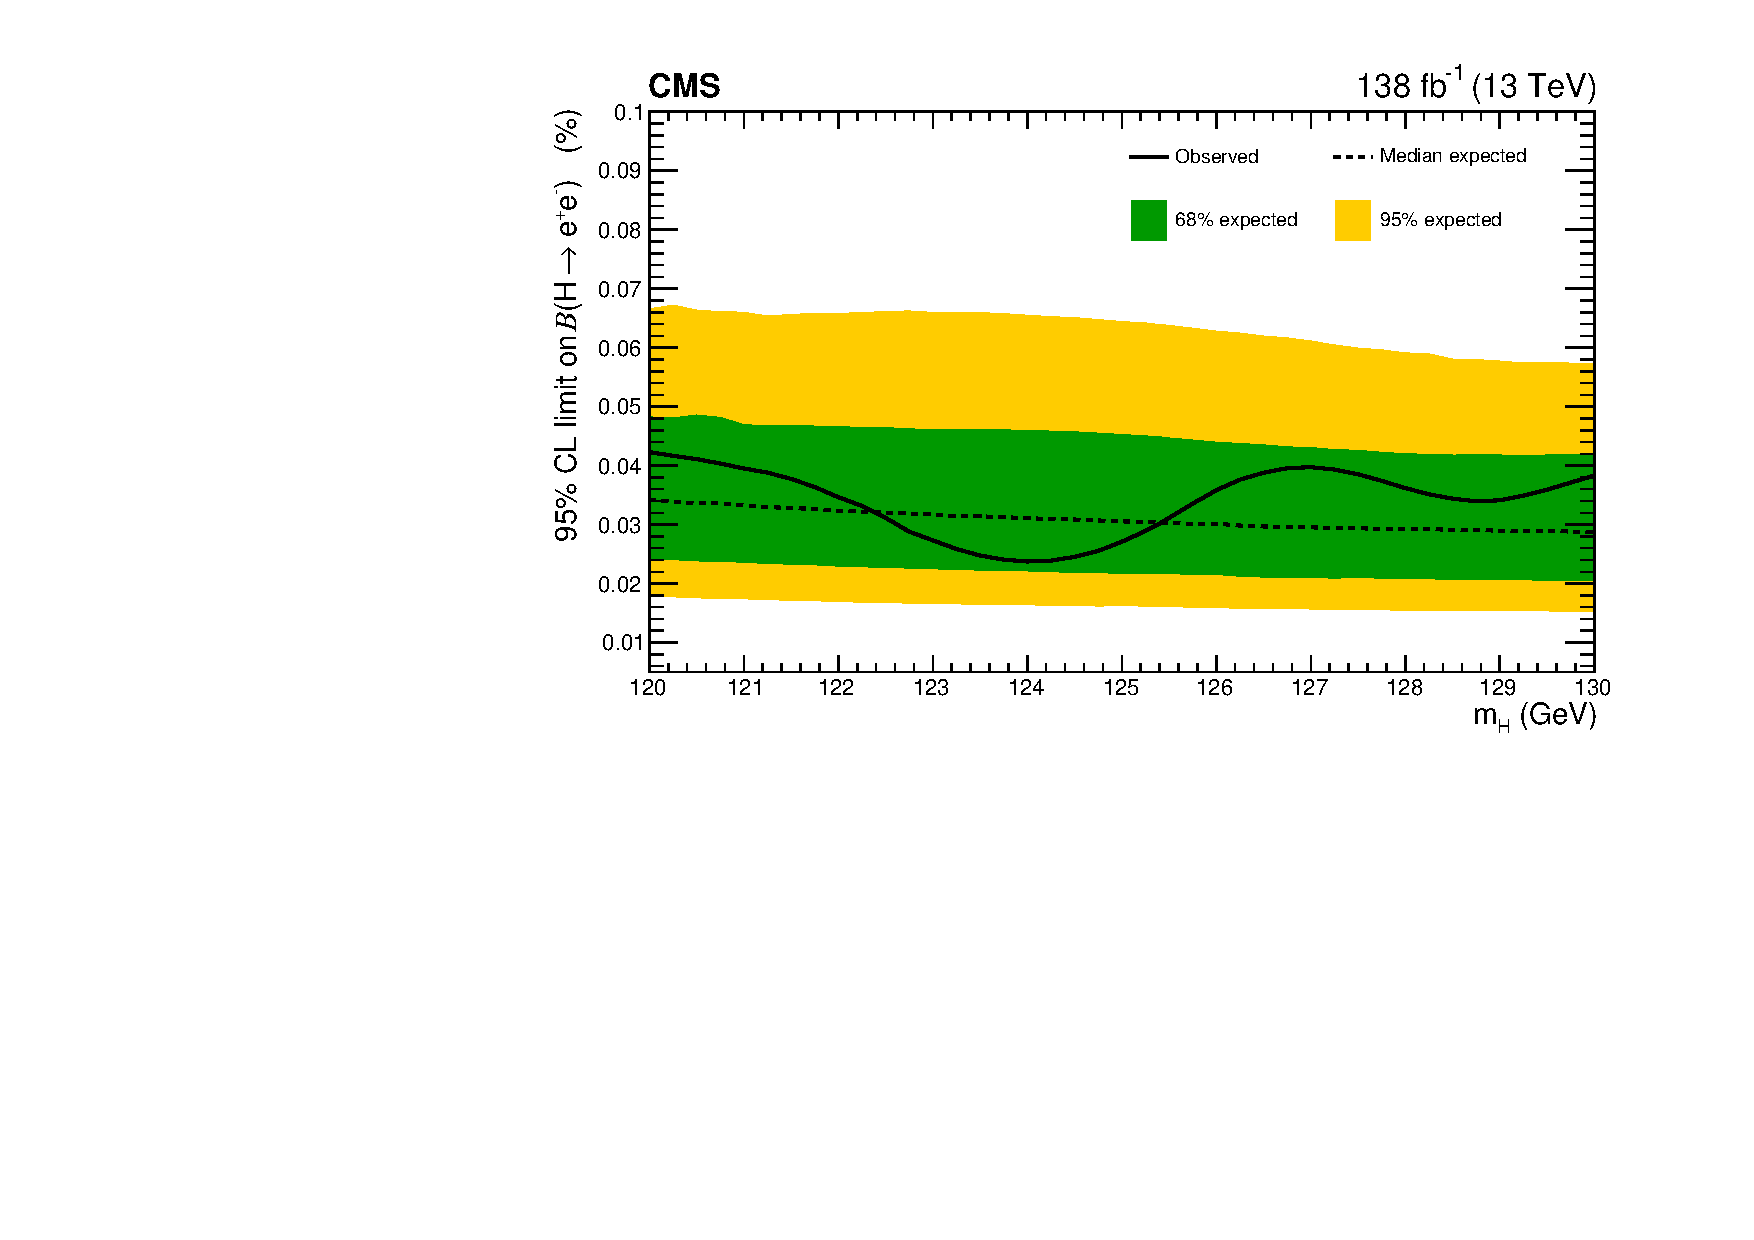
\includegraphics[width=0.8\textwidth]{Figures/Hee/Results/limits/limitVsMh_paper.pdf}\hfill%
\caption[Limits on \BHee as a function of the Higgs boson mass.]{Expected and observed limits on \BHee for Higgs boson masses between 120 and 130~GeV, along with the associated 1$\sigma$ (green) and 2$\sigma$ (yellow) CL intervals. The observed limits are within the 1$\sigma$ interval of the expected limits for all considered values of the Higgs boson mass.}
\label{fig:hee_limits}
\end{figure}


\begin{figure}[htbp!]
\centering
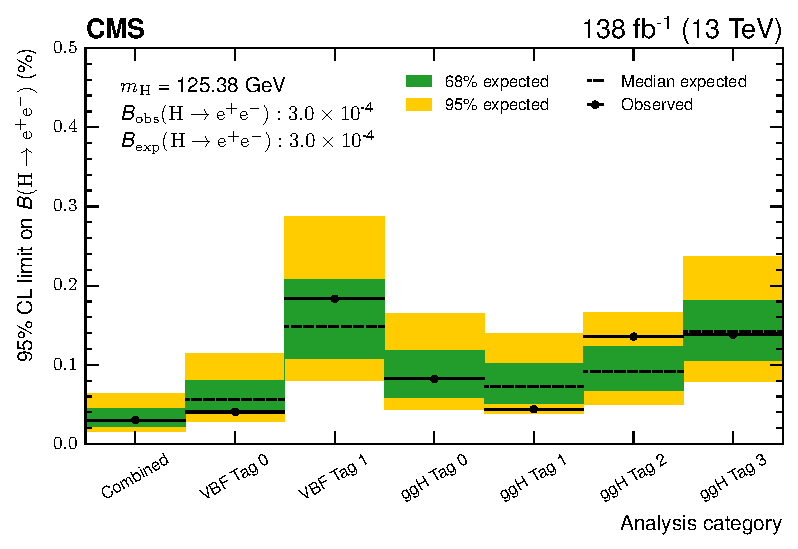
\includegraphics[width=0.75\textwidth]{Figures/Hee/Results/limits/per_category_limits_paper.pdf}\hfill%
\caption[Limits on \BHee per analysis category.]{Expected and observed limits on \BHee for each constructed analysis category, and all categories combined. The relative contribution to the overall sensitivity is similar between the most sensitive categories targeting \ggH and VBF events. The results here assume a SM Higgs boson with mass of 125.38~GeV. }
\label{fig:hee_limits_per_cat}
\end{figure}

\section{Summary}
\label{subsection:hee_s_b_models_summary}

The results of this analysis set exclusion limits on the branching fraction for \Hee decays. This is achieved using a maximum likelihood fit to the dielectron mass distribution across all analysis categories. Limits computed using the $\mathrm{CL}_s$ method are presented both as a function of the Higgs boson mass, and per analysis category. The contribution to the overall sensitivity from categories targeting \ggH and VBF production is similar in magnitude. For a nominal Higgs boson mass of 125.38~GeV, the observed (expected) limit at the 95\% CL on \BHee is found to be $3.0\times10^{-4}$ ($3.0\times10^{-4}$). Results are also translated into an upper limit on the Higgs boson effective coupling modifier to electrons, $|\kappa_{e}|$, which is found to be $|\kappa_{e}|<240$. These results provide the most sensitive constraints on the \Hee decay to date.